\documentclass{scrartcl}
\usepackage[utf8]{inputenc}
\usepackage[english]{babel}
\usepackage{caption}
\usepackage{subcaption}
\usepackage{listings}
\usepackage{pdfpages}
\usepackage{amsmath,amssymb}
\usepackage{siunitx}
\usepackage{hyperref}
\usepackage{mhchem}
\usepackage[section]{placeins}
\usepackage[activate, protrusion=true, expansion=true]{microtype}
\usepackage[left=2.5cm, right=2.5cm, bottom=2.5cm, top=2.5cm]{geometry}
\usepackage{libertine}
\usepackage{longtable}

\newcommand{\qed}{\hfill $\blacksquare$}
\newcommand{\gitlab}{\href{https://gitlab.lrz.de/arne/neuroprosthetics}{GitLab}}

\lstset{frame=single,keepspaces=true,captionpos=b}

\title{Case Study:\\Path Tracking for an Autonomous Vehicle}
\subtitle{Multivariate Control and Coordination Systems (EE-477)}
\author{\textsc{Arne Sachtler}}
\date{Lausanne, EPFL, 2018}

\begin{document}
\maketitle
\setcounter{section}{-1}
\section{Introduction}
The general objective of the case study is to follow a trajectory with the vehicle.
Trajectories are expressed in a parametric form, where a parameter $s$ specifies the displacement of the car on the trajectory.
Figure~\ref{fig:vehicle_model} shows the model and important parameters.
\begin{figure}[h]
	\centering
	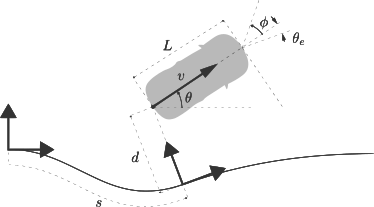
\includegraphics[width=.6\textwidth]{figures/model.pdf}
	\caption{Model of trajectories and the vehicle. Taken from the case study handout.}
	\label{fig:vehicle_model}
\end{figure}
For the dynamic equations several symbols are used. 
Table~\ref{tab:symbols} shows a summary of the symbols used within the document.
\begin{table}[h]
	\centering
	\begin{tabular}{c|l}
	\hline
	\hline
	\textbf{Symbol} & \textbf{Decription}\\
	\hline
		 $s$ & curvilinear coordinate\\
		 $d$ & lateral deviation between vehicle and path\\
		 $\theta_e$ & heading error\\
		 $v$ & longitudinal speed\\
		 $L$ & car length\\
		 $\phi$ & steering wheel angle\\
		 $\alpha$ & speed reference\\
		 $\beta$ & steering wheel angle reference\\
		 $\sigma_a, \sigma_s$ & dynamics of the actuators\\
		 $\kappa(s)$ & curvature of path at position s\\
	\hline
	\hline
	\end{tabular}
	\caption{Symbols used in the dynamics model of the vehicle}
	\label{tab:symbols}
\end{table}

\subsection*{State space model of the Vehicle}
The vehicle is modelled using a set of nonlinear differential equations in state space representation $\mathbf{\dot{x}} = \mathbf{f}(\mathbf{x}, \mathbf{u}, t)$.
The state vector of the system is defines as
\begin{equation}
	\mathbf{x} = \begin{bmatrix}
		x_1, &x_2, &x_3, &x_4, &x_5
	\end{bmatrix} = \begin{bmatrix}
		s, &d, &\theta_e, &v, &\phi
	\end{bmatrix}\, ,
\end{equation}
and the input
\begin{equation}
	\mathbf{u} = \begin{bmatrix}
		u_1, &u_2	
	\end{bmatrix} = \begin{bmatrix}
		\alpha, &\beta
	\end{bmatrix}\, .
\end{equation}
The model of the vehicle is provided in the case study handout
\begin{eqnarray}
	\dot{x_1} &=& \frac{x_4 \cos(x_3)}{1 - x_2\kappa}\\
	\dot{x_2} &=& x_4 \sin(x_3)\\
	\dot{x_3} &=& \frac{x_4}{L}\tan(x_5) - \frac{\kappa x_4 \cos(x_3)}{1 - x_2 \kappa}\\
	\dot{x_4} &=& \sigma_a (u_1 - x_4)\\
	\dot{x_5} &=& \sigma_s (u_2 - x_5)
\end{eqnarray}
\section{Linearization, Discretization and Simulation}

\end{document}
